\documentclass{article}

\usepackage{amsmath}
\usepackage{amssymb}
\usepackage{algorithm}
\usepackage{enumitem}
\usepackage[noend]{algpseudocode}		% for algorithms in pseudo code. Usage: \begin{algorithmic}
\MakeRobust{\Call}
\newcommand{\lang}{\mathcal{L}}
\usepackage{tikz}	% for diagrams
\usetikzlibrary{positioning}
\usetikzlibrary{quotes}

\setlength{\parskip}{\smallskipamount}

\title{Analysis of Algorithms \\
\medskip
\large Homework 7 -- \textit{NP}}
\author{Abraham Murciano \& Elad Harizy}

\begin{document}

\maketitle

\section{Subgraph Isomorphism}

We are given two graphs, \(G_1 = (V_1, E_1)\) and \(G_2 = (V_2, E_2)\). The subgraph isomorphism problem (SGI) is to determine if there exists a subgraph of \(G_2\) which is isomorphic to \(G_1\).

\subsection*{Part A}

To prove that \(\text{SGI} \in \mathit{NP}\) we must show that there is a way to verify a solution to the problem in polynomial time.

If we are given a solution to an SGI problem in the form of \(G_3 = (V_3, E_3)\), which is a subgraph of \(G_2\); and a bijection \(f : V_1 \to V_3\),which is a map from the vertices of \(G_1\) to the vertices of \(G_3\), then we can verify that they are in fact isomorphic as follows.

\begin{algorithm}
	\begin{algorithmic}
		\Function{Isomorphic}{$G_1, G_3, f$}
		\For{\((u, v) \in E_1\)}
		\If{\((f(u), f(v)) \notin E_3\)}
		\Return false
		\EndIf
		\EndFor
		\State \Return true
		\EndFunction
	\end{algorithmic}
\end{algorithm}

This algorithm is clearly \(O(E)\), so is polynomial. Therefore \(\mathit{SCI} \in \mathit{NP}\).

\subsection*{Part B}

To prove that SGI is \textit{NP}-complete, we will show that the Clique problem (which is known to be \textit{NP}-complete) is reducible to SGI.

The Clique problem is to determine, given a graph \(G = (V, E)\) and a constant \(c \leq |V|\), whether or not \(K_c\) (a complete graph with \(c\) vertices) is a subgraph of \(G\).

To reduce the Clique problem to SGI, we must convert every instance of the Clique problem into one of SGI, such that the solution will be the same for both. Consider some inputs to the Clique problem; a graph \(G\), and a constant \(c\). We can feed \(K_c\) and \(G\) as the inputs \(G_1\) and \(G_2\) of the SGI problem respectively. Then any SGI algorithm will tell us whether or not \(G = G_2\) has a subgraph isomorphic to \(K_c = G_1\), which is precisely the definition of the Clique problem.


\section{Simple Cycle Problem}

This problem is to find whether or not a given graph has a simple cycle (a cycle with no repeating vertices, other than the first and last) of \(k\) distinct vertices.

\subsection*{Part A}

This problem is in \textit{NP}. This can be easily shown since if we are given a cycle, we can walk the cycle and verify that there are precisely \(k\) vertices in linear time, and we can verify that they are all distinct in linear time with the use of a hash-set, or certainly in quadratic time by comparing all vertices to all previously seen ones. Therefore the problem is in \textit{NP}.

\subsection*{Part B}

We will now show that our problem is \textit{NP}-complete by showing that the Hamiltonian Cycle problem, which is known to be \textit{NP}-complete reduces to it.

The Hamiltonian Cycle problem goes as follows. Given a graph, is there a path that traverses all the vertices without repeating any, then ends back at the start?

For any instance of the Hamiltonian Cycle problem, supposing the input is the graph \(G = (V, E)\), we can construct an equivalent Simple Cycle problem by asking is there a simple cycle in \(G\) of \(k = |V|\) distinct vertices. If there is one, that is a hamiltonian cycle. Otherwise, there is no hamiltonian cycle. Thus the Simple Cycle problem is also \textit{NP}-complete.

\subsection*{Part C}

We are presented with another similar problem. Given a graph, does it contain \emph{any} cycles? This problem is different to the Simple Cycle problem, in that we do not care about the size of the cycle, nor do we care if there are smaller cycles within it.

This problem can be solved in polynomial time by performing a breadth-first search on the tree, and if back-edges are found, then there must be a cycle. Otherwise there cannot be one.

\section{Cliques and 3-CNF}

We are given the following boolean formula in 3-CNF.
\begin{align*}
	\varphi & = (a \lor b \lor \lnot c) \land (a \lor b \lor \lnot c) \land (\lnot a \lor \lnot b \lor c) \land (a \lor \lnot b \lor \lnot c) \\
	        & = (a \lor b \lor \lnot c) \land (\lnot a \lor \lnot b \lor c) \land (a \lor \lnot b \lor \lnot c)
\end{align*}

This boolean formula is solvable if and only if the graph in figure \ref{q3-clique} contains a clique of size three.

\begin{figure}[htbp]
	\centering
	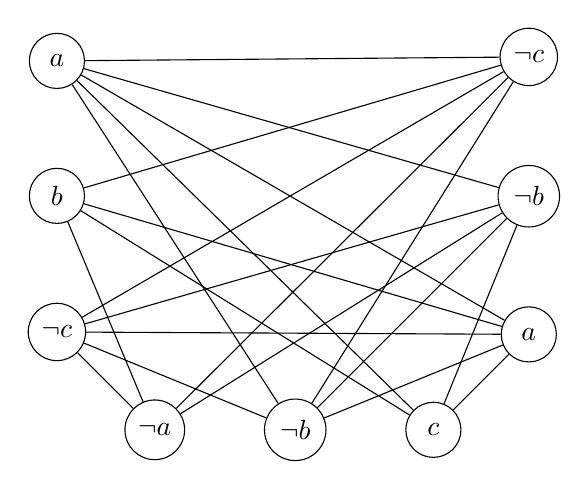
\begin{tikzpicture}
		[vertex/.style={circle, draw=black, node distance=1cm, minimum size=0.7cm}]
		\node[vertex] (a1) {\(a\)};
		\node[vertex, below=of a1] (b1) {\(b\)};
		\node[vertex, below=of b1] (c1) {\(\lnot c\)};

		\node[vertex, below right=of c1] (a2) {\(\lnot a\)};
		\node[vertex, right=of a2] (b2) {\(\lnot b\)};
		\node[vertex, right=of b2] (c2) {\(c\)};

		\node[vertex, above right=of c2] (a3) {\(a\)};
		\node[vertex, above=of a3] (b3) {\(\lnot b\)};
		\node[vertex, above=of b3] (c3) {\(\lnot c\)};

		\draw (a1) to (a3);
		\draw (a1) to (b2);
		\draw (a1) to (b3);
		\draw (a1) to (c2);
		\draw (a1) to (c3);

		\draw (b1) to (a2);
		\draw (b1) to (a3);
		\draw (b1) to (c2);
		\draw (b1) to (c3);

		\draw (c1) to (a2);
		\draw (c1) to (a3);
		\draw (c1) to (b2);
		\draw (c1) to (b3);
		\draw (c1) to (c3);

		\draw (a2) to (b3);
		\draw (a2) to (c3);

		\draw (b2) to (a3);
		\draw (b2) to (b3);
		\draw (b2) to (c3);

		\draw (c2) to (a3);
		\draw (c2) to (b3);
	\end{tikzpicture}
	\caption{A graph which contains a clique of size three iff \(\varphi\) is satisfiable.}
	\label{q3-clique}
\end{figure}

There are many cliques of size three in this graph, which means that there are many different ways to satisfy \(\varphi\). For example, figure \ref{q3-example} shows a few of the different cliques contained in the graph. If we take the red clique, that corresponds to the assignments \(a := \top, b := \bot\) in the context of the boolean formula \(\varphi\). Clearly, if we substitute these assignments into \(\varphi\), that would make \(\varphi = \top\), so it is obviously satisfiable.

\begin{figure}[htbp]
	\centering
	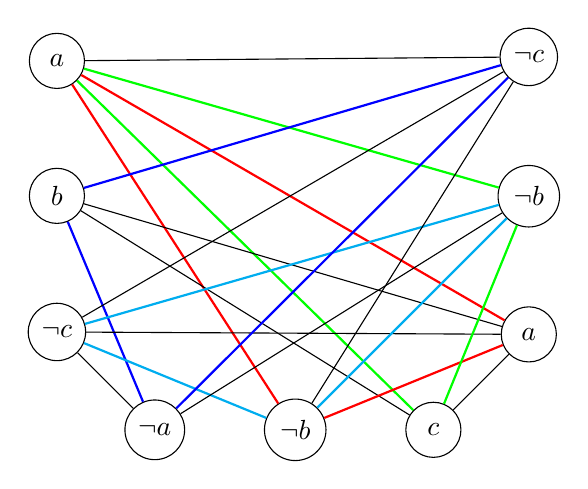
\begin{tikzpicture}
		[vertex/.style={circle, draw=black, node distance=1cm, minimum size=0.7cm}]
		\node[vertex] (a1) {\(a\)};
		\node[vertex, below=of a1] (b1) {\(b\)};
		\node[vertex, below=of b1] (c1) {\(\lnot c\)};

		\node[vertex, below right=of c1] (a2) {\(\lnot a\)};
		\node[vertex, right=of a2] (b2) {\(\lnot b\)};
		\node[vertex, right=of b2] (c2) {\(c\)};

		\node[vertex, above right=of c2] (a3) {\(a\)};
		\node[vertex, above=of a3] (b3) {\(\lnot b\)};
		\node[vertex, above=of b3] (c3) {\(\lnot c\)};

		\draw[thick, red] (a1) to (a3);
		\draw[thick, red] (a1) to (b2);
		\draw[thick, green] (a1) to (b3);
		\draw[thick, green] (a1) to (c2);
		\draw (a1) to (c3);

		\draw[thick, blue] (b1) to (a2);
		\draw (b1) to (a3);
		\draw (b1) to (c2);
		\draw[thick, blue] (b1) to (c3);

		\draw (c1) to (a2);
		\draw (c1) to (a3);
		\draw[thick, cyan] (c1) to (b2);
		\draw[thick, cyan] (c1) to (b3);
		\draw (c1) to (c3);

		\draw (a2) to (b3);
		\draw[thick, blue] (a2) to (c3);

		\draw[thick, red] (b2) to (a3);
		\draw[thick, cyan] (b2) to (b3);
		\draw (b2) to (c3);

		\draw (c2) to (a3);
		\draw[thick, green] (c2) to (b3);
	\end{tikzpicture}
	\caption{A graph which contains a clique of size three iff \(\varphi\) is satisfiable.}
	\label{q3-example}
\end{figure}

\section{Tasks and Machines}

We are given a set of \(n\) tasks with durations \(T = \{t_1, t_2, \dots, t_n\}\), a number of machines \(m\), and a time limit \(l\). All machines start at the same time, and continually process tasks until the time limit \(l\) is reached. The problem is to determine if all the tasks can be finished before the time limit.

\subsection*{Part A -- An Exponential Algorithm}

Algorithm \ref{q4-algo} which checks every possible way to perform the tasks, and returns true if it finds one that finishes on time. The complexity is \(O(n!)\), since there are \(n!\) permutations of \(T\).

\begin{algorithm}
	\begin{algorithmic}
		\Function{TasksAndMachines}{$T, m, l$}
		\For{each permutation \(P\) of \(T\)}
		\For{\(i\) from 1 to m} \Comment{Initialise working times of machines to 0}
		\State \(w_i := 0\)
		\EndFor
		\State \(i := 0\)
		\For{\(t \in P\)}
		\If{\(w_i + t < l\)} \Comment{Check if \(t\) fits on current machine's time}
		\State \(w_i := w_i + t\) \Comment{Reserve \(t\) time units on machine \(i\)}
		\Else
		\State \(i := i + 1\) \Comment{Move onto next machine}
		\If{\(i > m\)}
		\State Continue \Comment{No more machines. Try next permutation}
		\EndIf
		\State \(w_i := t\) \Comment{Reserve \(t\) time units}
		\EndIf
		\EndFor
		\State \Return True \Comment{This permutation fits in the time limit}
		\EndFor
		\State \Return False \Comment{No permutations were found to fit}
		\EndFunction
	\end{algorithmic}
	\caption{}
	\label{q4-algo}
\end{algorithm}

\subsection*{Part B}

This problem is in \textit{NP}, since if we are given a partitioning of \(T\) into at most \(m\) partitions, we can verify that the sum of each partition is less than \(l\), and we would know that indeed, each partition can be assigned to one machine, and they would all finish before the time limit. This can be checked in polynomial time.

\subsection*{Part C -- Reduction from the Bin Packing Problem}

In the bin packing problem, \(n\) items of different volumes \(V = \{v_1, v_2, \dots, v_n\}\) must be packed into \(k\) bins or containers, each of a fixed given volume \(b\). It is known that the bin packing problem is \textit{NP}-complete.

Now to reduce the bin packing problem to our problem, we first create a task for each item whose duration is the same as the volume of the corresponding item; formally, \(\forall 1 \leq i \leq n, (t_i = v_i)\). We then set the time limit \(l\) to be equal to the volume of each bin \(b\). Finally, we set the number of machines to the number of bins available.

Now we are able to partition the tasks into partitions for each machine, if and only if we are able to partition the items into bins.

\end{document}